\chapter{Approccio proposto}
\label{chap:approccio}
\vspace{1cm}
Nel Capitolo \ref{chap:SOA} sono state descritte alcune soluzioni proposte 
relative al lavoro oggetto di questa tesi, in particolare algoritmi esatti ed
euristici di ottimizzazione basati su varie tecniche.
% TODO & FIXME aggiungere qualcosa (tipo pro/contro)

In questo capitolo verrà descritto l'approccio utilizzato per risolvere il 
problema di scheduling dei task tenendo in considerazione le comunicazioni e 
riconfigurazioni introdotte.

Il capitolo è organizzato secondo la seguente struttura: nella Sezione 
\ref{sec:integrazioneToolchainFASTER} viene descritta l'integrazione 
dell'algoritmo di scheduling con il componente che gestisce il mapping dei task, 
con accenni alle interfacce esterne che collegano il componente 
con gli altri strumenti utilizzati nella toolchain di \acs{FASTER}; la Sezione 
\ref{sec:panoramicaMetodologia} descrive ad alto livello il funzionamento 
dell'algoritmo di scheduling, fornendo una panoramica delle fasi in cui questo 
si divide; la Sezione \ref{sec:euristicaSceltaTask} contiene una descrizione 
dettagliata della fase più delicata del procedimento di scheduling, la scelta 
del task migliore da considerare ad ogni passo di decisione; la Sezione 
\ref{sec:osservazioniConclusive} fornisce un riepilogo dei concetti importanti 
presentati in questo capitolo.


\section{Integrazione nella toolchain di \acs{FASTER}}
\label{sec:integrazioneToolchainFASTER}

Come descritto nel precedente capitolo, l'obiettivo del progetto europeo 
\ac{FASTER} è fornire un framework per la sintesi ad alto livello di 
applicazioni, scritte in linguaggio di programmazione C, su vari dispositivi 
riconfigurabili; la toolchain che permette di realizzare questa sintesi è 
composta da varie fasi eseguite in sequenza. Ogni fase deve essere il più 
possibile self-contained, ovvero deve poter essere invocata separatamente e non 
deve avere nozioni sul funzionamento interno delle altre fasi.

Condizione necessaria perchè ciò accada è la definizione di specifiche 
interfacce per ogni strumento che deve essere invocato. Ad esempio, la fase di 
mapping ha la propria interfaccia di input e di output; lo scheduler 
(incapsulato nell'algoritmo evolvibile di esplorazione delle soluzioni) ha 
anch'esso una interfaccia di input e una di output, contenenti tutte 
le strutture dati necessarie per l'elaborazione e per la memorizzazione delle 
informazioni calcolate dall'algoritmo, rispettivamente. 

%%% FIXME: color
\begin{figure}
 \begin{center}
  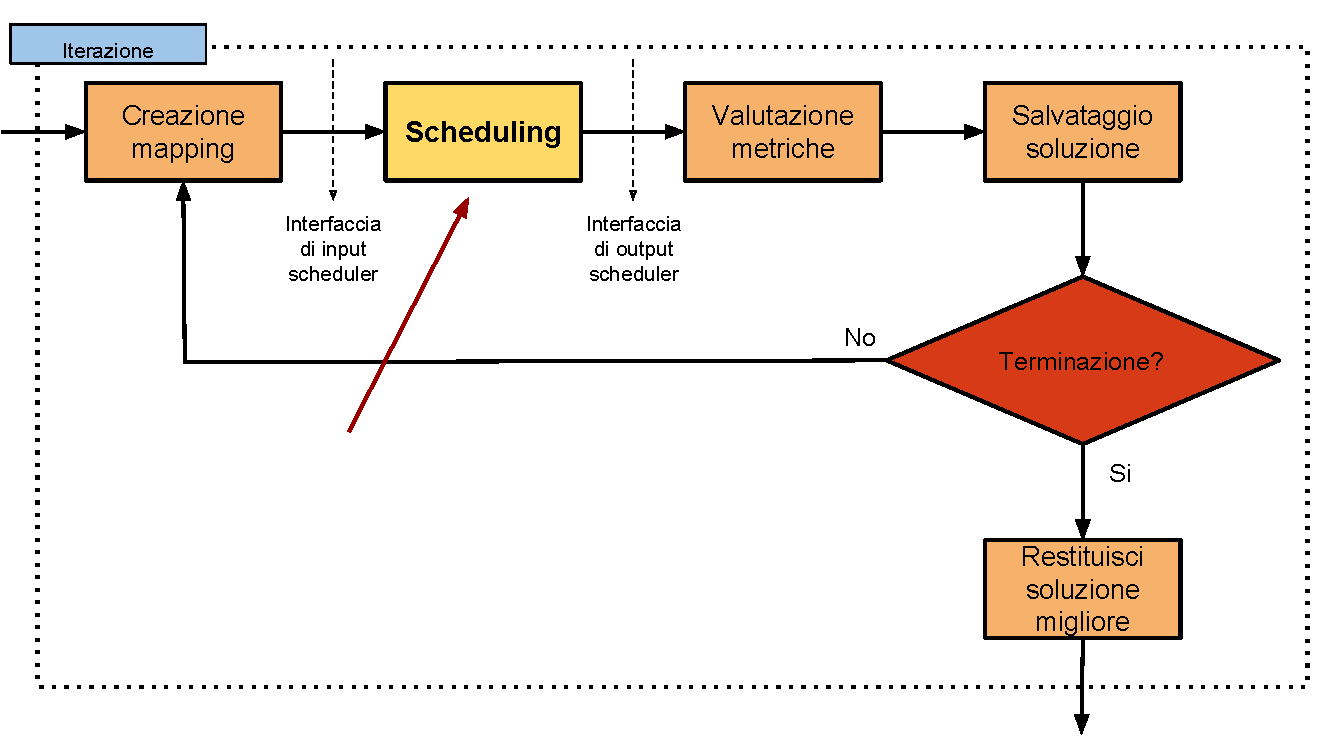
\includegraphics[width=0.9\textwidth]{capitoli/figure/cap3/MapperWorkflow.pdf}
  \caption{Flusso di lavoro dell'algoritmo di esplorazione.}
  \label{fig:mapperWorkflow}
 \end{center}
\end{figure}

A livello dell'algoritmo di esplorazione delle soluzioni, dunque, si avrà un 
flusso di lavoro come rappresentato nella Figura \ref{fig:mapperWorkflow}, in 
cui è messo in evidenza dove si colloca la fase di scheduling oggetto del 
lavoro, con le relative interfacce di input e output.

Anche la fase di mapping, che precede l'invocazione del tool che gestisce lo 
scheduling, è caratterizzata dalle proprie interfacce di input e output. Come 
si può vedere nella Figura \ref{fig:mapperWorkflow}, poichè la fase di 
scheduling è immediatamente successiva a quella di mapping, l'interfaccia di 
output del mapper e l'interfaccia di input dello scheduler avranno alcuni dati 
in comune.


\subsection{Interfaccia di input}

%%%%%%%%%%%% FIXME %%%%%%%%%%%%%
%%% overfull hbox %%%
\begin{figure}
 \begin{minipage}[b]{0.4\textwidth}
  \begin{center}
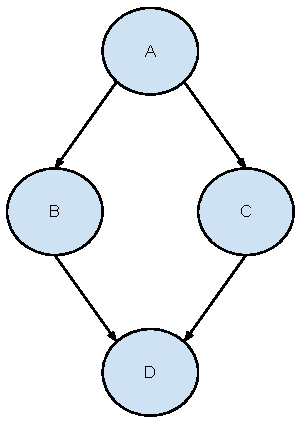
\includegraphics[width=\linewidth]{capitoli/figure/cap3/TaskGraphExample.pdf}
  \subcaption{Task graph}\label{fig:taskGraphExample2}
  \end{center}
 \end{minipage}
 \hfill
 \begin{minipage}[b]{0.4\textwidth}
  \begin{center}
   \begin{tabular}{| c | c | c |}
    \hline
    \textbf{Task} & \textbf{Component} & \textbf{Implementation}\\
    \hline
    A & p1 & impl\textunderscore0\\
    \hline
    B & p2 & impl\textunderscore1\\
    \hline
    C & p1 & impl\textunderscore2\\
    \hline
    D & p3 & impl\textunderscore3\\
    \hline
   \end{tabular}
   \subcaption{Lista dei mapping}\label{tab:listaMapping}
  \end{center}
 \end{minipage}
 \caption{Esempio di task graph e di lista dei mapping.}
 \label{fig:taskGraphAndMapping}
\end{figure}


L'interfaccia di input per la fase di scheduling contiene tutti i dati 
necessari all'esecuzione dello scheduler, alcuni definiti prima 
dell'invocazione del tool, altri creati o modificati durante le differenti fasi 
dell'esecuzione. In particolare, i dati definiti prima dell'invocazione sono:
\begin{itemize}
 \item dati provenienti dal file XML di specifica del progetto correntemente in 
elaborazione dalla toolchain, relativi alla descrizione dell'architettura, del 
task graph, delle implementazioni e dei vari elementi 
di computazione, di 
comunicazione e di memoria presenti;
 \item dati provenienti dall'output della fase di mapping.
\end{itemize}
Questi ultimi sono organizzati come una lista di triple \emph{$<$processing 
task, processing element, implementazione$>$} calcolata dal mapper, che 
specifica per ogni task:
\begin{enumerate}
 \item l'elemento di computazione che dovrà eseguire il task, può essere un 
core hardware su scheda oppure un soft core (processore);
 \item l'implementazione da utilizzare per l'esecuzione del task, si può 
dividere in implementazione software o hardware a seconda che il task debba 
essere eseguito su scheda o su un processore.
\end{enumerate}
Nella Figura \ref{fig:taskGraphAndMapping} sono rappresentati un esempio di 
task graph e di output della fase di mapping basato su quel task graph.

Le informazioni provenienti dal mapper vengono quindi utilizzate per 
determinare se alcune aree dovranno essere riconfigurate durante l'esecuzione 
dell'applicazione oppure no, oltre a dare informazioni sull'occupazione dei 
vari componenti del dispositivo.


\subsection{Interfaccia di output}

Il compito dello scheduler è assegnare delle stime di tempo di inizio e di fine 
esecuzione ad ogni task in modo che le precedenze tra i task imposte dal task 
graph vengano rispettate, e che nessun altro vincolo sia violato: ad esempio, 
task che devono essere eseguiti sullo stesso componente non possono avere tempi 
di esecuzione sovrapposti. Tutte queste informazioni sulle stime calcolate 
dallo scheduler vengono memorizzate nell'interfaccia di output, che è composta 
da:
\begin{itemize}
 \item una rappresentazione in forma di \emph{diagramma di Gantt}, che delinea 
per ogni componente quando questo è occupato nell'esecuzione di un task;
 \item per ogni task, una lista delle informazioni riguardanti lo scheduling, 
ad esempio il tempo d'esecuzione stimato, il componente su cui deve essere 
eseguito, l'implementazione che ne caratterizza l'esecuzione e le stime di 
inizio e fine esecuzione che gli sono state assegnate.
\end{itemize}

Nella prossima sezione verrà spiegato in dettaglio il flusso di 
esecuzione dell'algoritmo di scheduling e come le interfacce vengono 
utilizzate durante l'elaborazione.


\section{Panoramica della metodologia}
\label{sec:panoramicaMetodologia}

In questa sezione viene descritto il funzionamento dell'algoritmo proposto e le 
fasi in cui esso si articola, con una spiegazione dettagliata della struttura 
di ogni fase e del flusso di lavoro completo dell'algoritmo.

Come accennato nella sezione precedente, l'interfaccia di input è 
caratterizzata da dati ``statici'', presenti prima dell'invocazione dello 
scheduler e da dati ``dinamici'', che subiscono modifiche oppure vengono creati 
durante l'esecuzione del tool. L'interfaccia di output è invece costruita 
incrementalmente, aggiungendo e modificando dati man mano che la computazione 
prosegue.


\begin{figure}[ht]
 \begin{center}
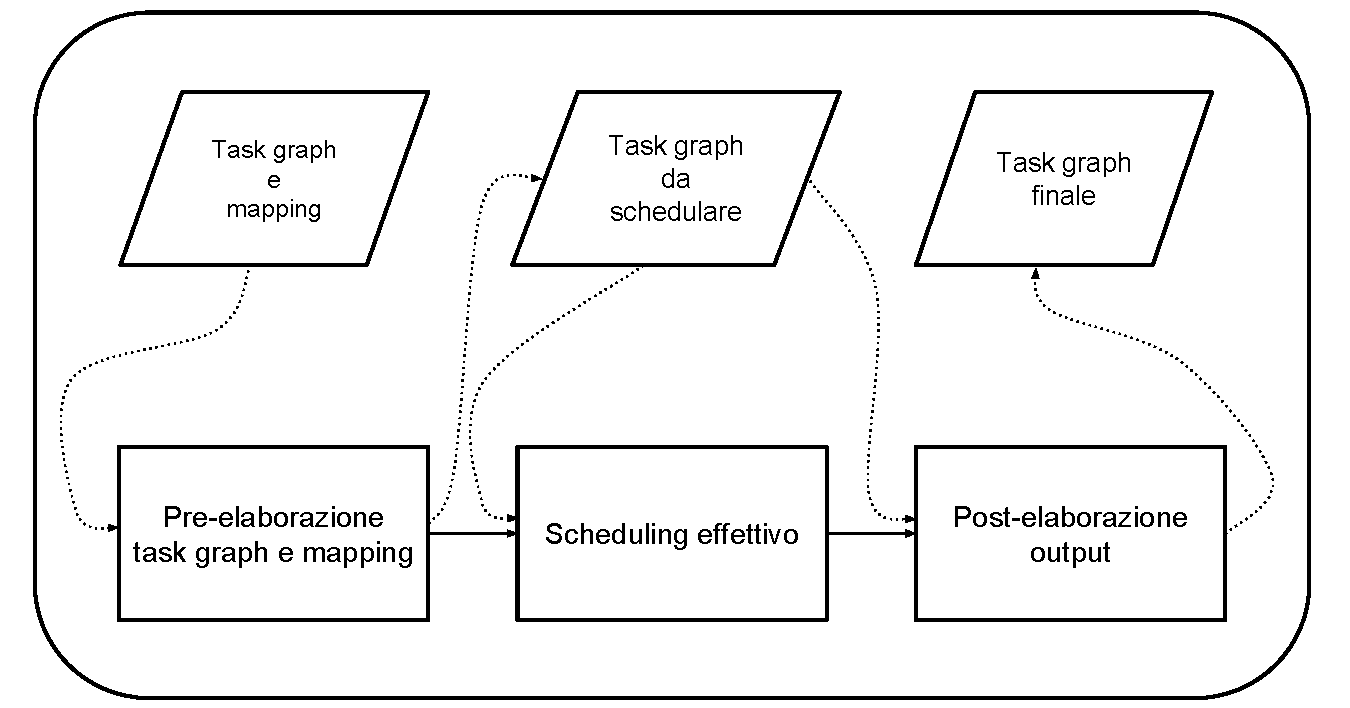
\includegraphics[width=0.9\textwidth]
{capitoli/figure/cap3/SchedulerWorkflow.pdf}
  \caption{Flusso di lavoro dell'algoritmo di scheduling.}
  \label{fig:schedulerWorkflow}
 \end{center}
\end{figure}


La prima fase dell'algoritmo ha il compito di 
effettuare una elaborazione preliminare dei dati statici, che permetterà di 
ottenere una formulazione più specifica e dettagliata del problema; questa 
prima fase è chiamata \emph{fase di preprocessing}. La seconda fase è 
costituita dallo \emph{scheduling effettivo} dei task, utilizzando le 
informazioni calcolate in precedenza nella pre-elaborazione. La terza e ultima 
fase, pur non essendo strettamente legata all'assegnazione delle stime dei tempi 
e dell'ordine di esecuzione dei task, è fondamentale per permettere l'effettiva 
esecuzione dell'applicazione sul dispositivo riconfigurabile; consiste in una 
parziale rielaborazione dell'output prodotto dalla fase di scheduling ed è 
chiamata \emph{fase di postprocessing}.

Le tre fasi sono rappresentate nella Figura \ref{fig:schedulerWorkflow}, che 
illustra il flusso di lavoro dello scheduler, con i relativi dati di input per 
ogni fase. Nelle prossime sezioni, ogni fase verrà analizzata nel dettaglio.


\subsection{Fase di preprocessing}
La fase di preprocessing è la prima ad essere eseguita dopo l'invocazione del 
tool di scheduling da parte dell'algoritmo di esplorazione. Ha come obiettivo 
principale l'identificazione delle comunicazioni e delle riconfigurazioni che 
devono essere prese in considerazione per la corretta esecuzione 
dell'applicazione sul dispositivo. Un obiettivo secondario è il calcolo di 
informazioni aggiuntive che verranno poi utilizzate nella fase di scheduling 
per quanto concerne la scelta del task migliore (vedi Sezione 
\ref{sec:euristicaSceltaTask}).

Per ottenere questi obiettivi, la fase di preprocessing si divide in tre 
sotto-fasi eseguite nel seguente ordine:
\begin{enumerate}
 \item aggiunta delle comunicazioni: nuovi task, detti \emph{task di 
comunicazione} vengono aggiunti al task graph originale, a rappresentare le 
comunicazioni che si verificano tra i task di computazione;
 \item aggiunta delle riconfigurazioni: può non essere richiesto e dipende 
dagli assegnamenti stabiliti dal mapping, consiste nell'introduzione di nuovi 
task, detti \emph{task di riconfigurazione}, dove necessario;
 \item computazione delle informazioni sul percorso critico.
\end{enumerate}

\subsubsection{Aggiunta delle comunicazioni}
L'inserimento dei task di comunicazione viene fatto solamente in base 
all'analisi del task graph dell'applicazione, in quanto indipendente dal 
mapping: dato che ogni arco in tale grafo rappresenta una relazione 
produttore-consumatore tra due task\footnote{Ovvero, denominati $i$ e $j$ i due 
task, un arco $(i,j)$ indica che l'output della computazione del task $i$ viene 
utilizzato come input per la computazione del task $j$.}, ogni arco viene 
trattato come una comunicazione.

Dati due task di computazione $i$, $j$ e un 
arco $(i,j)$ nel task graph, vi sono due tipi di task di comunicazione, che si 
differenziano per come operano il trasferimento dei dati:
\begin{itemize}
 \item task di comunicazione di tipo \emph{WRITE}, che \emph{scrivono} 
l'output del task $i$ in una memoria;
 \item task di comunicazione di tipo \emph{READ}, che \emph{leggono} dei dati 
da una memoria e li trasferiscono come input per il task $j$. 
\end{itemize}
Stanti queste premesse, ogni arco nel task graph implica l'inserimento di 
entrambi i tipi di task di comunicazione. L'arco originale viene rimosso e 
sostituito con nuovi archi che collegano i task di computazione con i task di 
comunicazione appena inseriti, rispettando i criteri precedentemente stabiliti.


\begin{figure}
 \begin{minipage}[b]{0.4\textwidth}
  \begin{center}
   $\vcenter{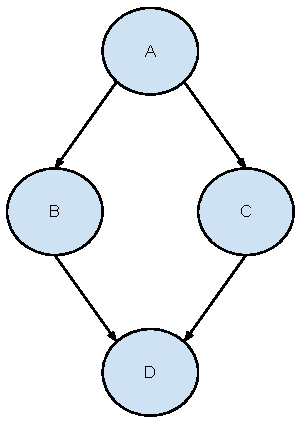
\includegraphics[width=\linewidth]
{capitoli/figure/cap3/TaskGraphExample.pdf}}$
  \end{center}
 \end{minipage}
 \hfill
 \begin{minipage}[b]{0.4\textwidth}
 \begin{center}
    $\vcenter{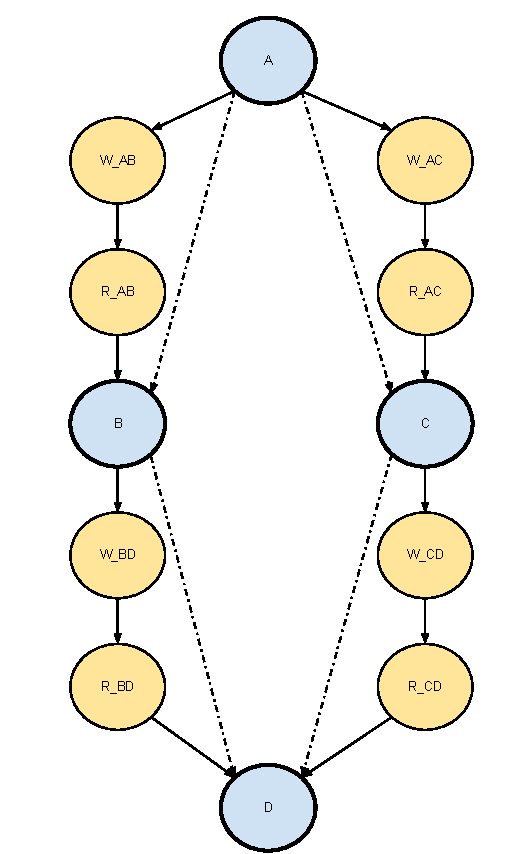
\includegraphics[width=\linewidth]
{capitoli/figure/cap3/TaskGraphCommunicationExample.pdf}}$
 \end{center}
 \end{minipage}
 \caption{Modifica del task graph in seguito all'aggiunta delle 
comunicazioni.}
 \label{fig:taskGraphCommunicationExample}
\end{figure}


Si veda la Figura \ref{fig:taskGraphCommunicationExample}
per un esempio di come viene modificato il task graph della Figura 
\ref{fig:taskGraphExample2} in seguito all'aggiunta dei task di 
comunicazione\footnote{Gli archi del grafo originale sono stati 
tratteggiati per evidenziare come la struttura generale non sia cambiata ma 
siano stati soltanto introdotti nuovi nodi e archi nel grafo.}.

Dopo l'inserimento dei task di comunicazione, viene eseguito l'inserimento dei 
task di riconfigurazione, qualora il particolare mapping utilizzato lo 
richieda. Nel caso, si procede come descritto nel prossimo paragrafo.


\subsubsection{Aggiunta delle riconfigurazioni}
L'inserimento dei task di riconfigurazione avviene in seguito all'analisi della 
lista dei mapping fornita dal mapper ed è necessario nel caso in cui gli 
assegnamenti stabiliti dal mapper verifichino le seguenti condizioni:
\begin{enumerate}
 \item due task di comunicazione sono mappati sullo stesso componente 
(processing element);
 \item le implementazioni dei due task sono diverse e di tipo hardware, ovvero 
i due task devono essere eseguiti su logica riconfigurabile: questa condizione 
implica che il modulo hardware non sia riutilizzabile da parte del secondo task.
\end{enumerate}
Se queste condizioni sussistono per una qualsiasi coppia di task, allora 
un nuovo task di riconfigurazione deve essere aggiunto al grafo. Nella Tabella 
\ref{tab:esempioRiconfigurazione} è illustrato un esempio di quando si 
verificano le precedenti condizioni ed è necessario introdurre un nuovo task di 
riconfigurazione.

\begin{table}
\begin{center}
\begin{tabular}{| c | c | c |}
 \hline
    \textbf{Task} & \textbf{Component} & \textbf{Implementation}\\
    \hline
    A & \textcolor{red}{p1} & \textcolor{blue}{impl\textunderscore0}\\
    \hline
    B & p2 & impl\textunderscore1\\
    \hline
    C & \textcolor{red}{p1} & \textcolor{blue}{impl\textunderscore2}\\
    \hline
    D & p3 & impl\textunderscore3\\
    \hline
\end{tabular}
\caption{Esempio di riconfigurazione necessaria.}
\label{tab:esempioRiconfigurazione}
\end{center}
\end{table}


L'inserimento avviene seguendo un preciso criterio per l'introduzione delle 
dipendenze: non si può semplicemente inserire il nuovo task tra i due task di 
computazione e collegarlo a questi con dei nuovi archi, è necessario tenere 
conto delle comunicazioni appena introdotte. Ad esempio, dati due task di 
computazione $i$ e $j$ anche non adiacenti, non è possibile eseguire la 
riconfigurazione prima che l'output del task $i$ sia stato salvato in memoria 
perchè i dati sarebbero sovrascritti e non più disponibili; allo stesso tempo 
e per il medesimo motivo, non è possibile eseguirla dopo che i dati siano stati 
trasferiti come input per il task $j$. Questi vincoli determinano i seguenti
criteri di assegnazione delle precedenze:
\begin{itemize}
 \item nuovi archi sono introdotti da tutti i task di comunicazione di tipo 
\emph{WRITE} uscenti dal task $i$ al task di riconfigurazione;
 \item nuovi archi sono introdotti dal task di riconfigurazione a tutti i task 
di comunicazione di tipo \emph{READ} entranti nel task $j$.
\end{itemize}


\begin{figure}
 \begin{minipage}[b]{0.4\textwidth}
$\vcenter{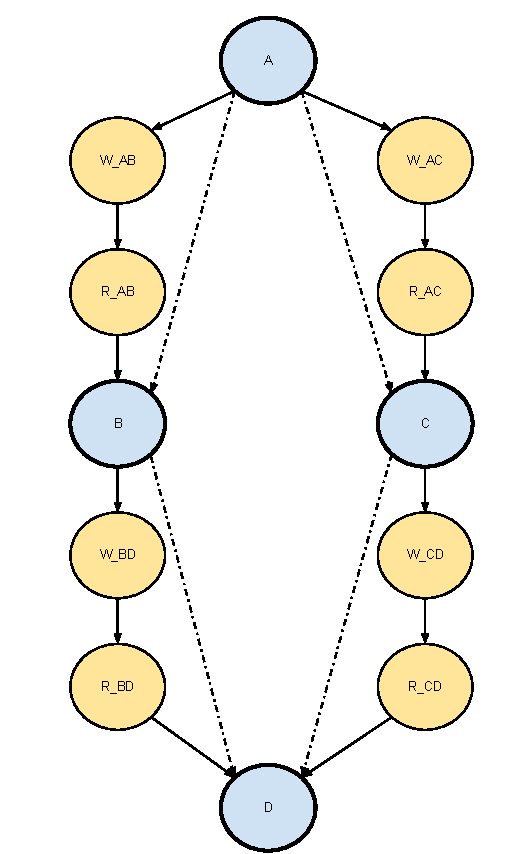
\includegraphics[width=\linewidth]
{capitoli/figure/cap3/TaskGraphCommunicationExample.pdf}}$
 \end{minipage}
 \hfill
 \begin{minipage}[b]{0.4\textwidth}
$\vcenter{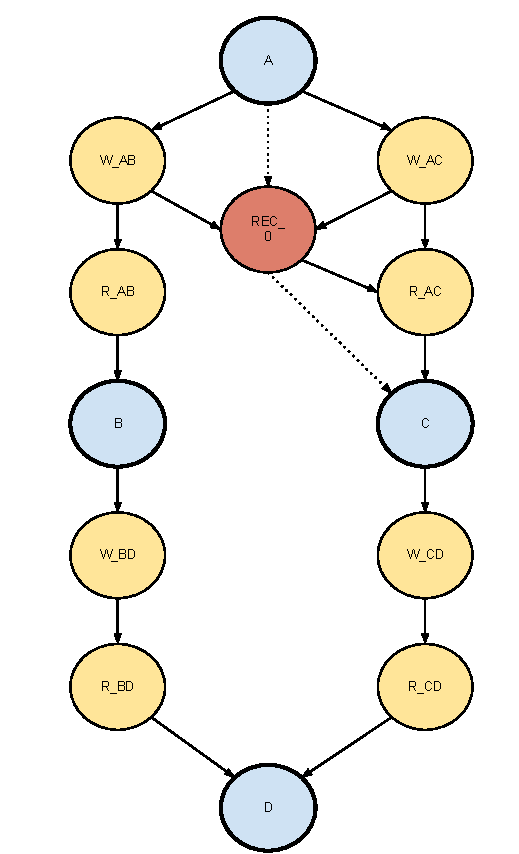
\includegraphics[width=\linewidth]
{capitoli/figure/cap3/TaskGraphCommRecExample.pdf}}$
 \end{minipage}
 \caption{Modifica del task graph in seguito all'aggiunta delle 
riconfigurazioni.}
 \label{fig:taskGraphCommRecExample}
\end{figure}


Nella Figura \ref{fig:taskGraphCommRecExample} è rappresentata l'evoluzione del 
task graph successiva all'introduzione dei task di riconfigurazione, sulla 
base dei mapping riportati nella Figura \ref{tab:listaMapping} e nella
Tabella \ref{tab:esempioRiconfigurazione}. Si può vedere il nuovo task di 
riconfigurazione introdotto, di colore rosso; gli archi entranti e uscenti dal 
nuovo task impongono le precedenze sopra elencate.

Una considerazione 
aggiuntiva riguarda gli archi tratteggiati che, nel grafo sulla destra, 
collegano i due task di computazione con il task di riconfigurazione: questi 
archi vengono inseriti in ogni caso durante il preprocessing, per esplicitare 
che deve verificarsi una riconfigurazione tra l'esecuzione del task $A$ e 
l'esecuzione del task $C$. La loro introduzione non influenza tuttavia il 
funzionamento dello scheduler. Le precedenze aggiuntive introdotte dal cammino 
$A \rightarrow REC\_0 \rightarrow C$ sono infatti dominate dai cammini già 
esistenti $A \rightarrow W\_AC \rightarrow REC\_0 \rightarrow R\_AC \rightarrow 
C$ e $A \rightarrow W\_AB \rightarrow REC\_0 \rightarrow R\_AC \rightarrow C$, 
quindi la presenza di tali archi non introduce nessun ritardo e non comporta 
svantaggi rispetto alla loro assenza.

Dopo l'aggiunta dei task di riconfigurazione, l'ultimo passo della fase di 
preprocessing consiste nel calcolo delle informazioni sul percorso critico del 
task graph.


\subsubsection{Calcolo delle informazioni sul percorso critico}
Le informazioni calcolate durante questa fase vengono utilizzate per stabilire 
quali task sono sul percorso critico\footnote{In inglese \emph{critical path}, 
avendo un grafo che simboleggia un progetto composto da attività (nodi) con 
precedenze (archi), rappresenta un cammino dal nodo iniziale al nodo finale del 
grafo costituito da attività che non possono essere ritardate senza allungare 
il tempo di esecuzione del progetto.}; verranno poi utilizzate nella fase di 
scheduling vero e proprio per l'assegnazione della priorità ai task

Tali informazioni consistono in tre dati, calcolati per ogni task del grafo 
preprocessato:
\begin{itemize}
 \item istante al più presto \emph{(asap)},
 \item istante al più tardi \emph{(alap)},
 \item scarto \emph{(slack)}: differenza tra istante al più tardi e istante al 
più presto.
\end{itemize}
I task con scarto pari a $0$ fanno parte del percorso critico.

Il calcolo delle tre informazioni sopra elencate viene effettuato tramite un 
semplice algoritmo comunemente utilizzato in ricerca operativa: il \ac{CPM}.
Vengono quindi aggiunti due \emph{nodi dummy}: sorgente, collegato ai nodi del 
grafo senza predecessori e destinazione, collegato ai nodi senza successori.
Il grafo viene poi ordinato topologicamente\footnote{Si noti che il task graph 
è aciclico quindi l'ordinamento topologico è sempre possibile.}, e l'algoritmo 
\ac{CPM} viene eseguito. Lo pseudocodice dell'algoritmo di ordinamento 
topologico è illustrato nell'Algoritmo \ref{alg:CPM}, dove $\delta^-(i)$ e 
$\delta^+(i)$ rappresentano il taglio entrante e il taglio uscente del nodo 
$i$, rispettivamente.

\IncMargin{1em}
\begin{algorithm}
 \SetKwInOut{Input}{input}\SetKwInOut{Output}{output}
 \SetKwArray{Asap}{asap}\SetKwArray{Alap}{alap}
 \SetKw{KwDownTo}{downto}
 
 \Input{Un grafo $G=(N,A)$, con $n = \vert N \vert$ e $d_i,\; \forall i = 
1,\dots,n$ durata del task $i$}
 \Output{$asap[i]$ e $alap[i],\; \forall i = 1,\dots, n$}
 \BlankLine
 \Asap{1} $\leftarrow 0$\;
 \For{$i = 2$ \KwTo $n$}{
 \Asap{i} $\leftarrow max\{$\Asap{p}$+ d_p\;:\;(p,i) \in \delta^-(i)\}$\;
 }
 \Alap{n} $\leftarrow$ \Asap{n}\;
 \For{$i=n-1$ \KwDownTo $1$}{
 \Alap{i} $\leftarrow min\{$\Alap{t}$- d_i\;:\;(i,t) \in \delta^+(i)\}$\;
 }
 \caption{Algoritmo CPM}
\label{alg:CPM}
\end{algorithm}
\DecMargin{1em}

Il calcolo delle informazioni sul percorso critico conclude la fase di 
preprocessing. Al termine di questa fase, il task graph presente 
nell'interfaccia di input dello scheduler viene sostituito con il grafo 
arricchito di comunicazioni e riconfigurazioni; le informazioni sul percorso 
critico appena calcolate sono aggiunte all'interfaccia, per essere utilizzate 
dalla fase successiva.


\subsection{Fase di scheduling}
La fase di scheduling effettivo gestisce l'assegnazione di tempi di inizio e 
fine dell'esecuzione di ogni task, sia esso di computazione, comunicazione o 
riconfigurazione. In particolare, a condizione che le stime sulla durata dei 
task siano il più precise possibile, la fase di scheduling assegna un ordine di 
esecuzione dei task che rispetti tutte le precedenze imposte dal task graph e 
che cerchi di minimizzare il tempo di esecuzione \emph{stimato}.

\IncMargin{1em}
\begin{algorithm}
 \SetKwInOut{Input}{input}\SetKwInOut{Output}{output}
 \SetKwData{UnscheduledSet}{unscheduledSet}
 \SetKwData{SchedulerOutput}{schedulerOutput }
 \SetKwData{SchedulerInput}{schedulerInput}
 \SetKwData{BestTask}{bestTask}
 \SetKwData{ReadyTaskSet}{readyTaskSet}
 \SetKwData{TimeInfo}{timeInfo}
 
 \Input{the input interface of the scheduler}
 \Output{the output interface of the scheduler}
 \BlankLine
 \SchedulerOutput $\leftarrow \emptyset$\;
 \UnscheduledSet $\leftarrow$ \SchedulerInput.getTaskSet()\;
 \While{\UnscheduledSet is not empty}{
 \ReadyTaskSet $\leftarrow$ tasks with precedences satisfied\;
 \BestTask $\leftarrow$ best task to be scheduled among the ready tasks\;
 \TimeInfo $\leftarrow$ compute start/end time estimations for the best task\;
 \SchedulerOutput $\leftarrow$ \SchedulerOutput $\cup$ \TimeInfo\;
 \ReadyTaskSet $\leftarrow$ \ReadyTaskSet $\setminus$ \BestTask\;
 \UnscheduledSet $\leftarrow$ \UnscheduledSet $\setminus$ \BestTask\;
 }
 \Return{\SchedulerOutput}
\caption{Algoritmo per la fase di scheduling}
\label{alg:faseScheduling}
\end{algorithm}
\DecMargin{1em}

Lo pseudocodice della fase di scheduling proposta è raffigurato nell'Algoritmo 
\ref{alg:faseScheduling}.


\subsection{Fase di postprocessing}


\section{Euristica di scelta dei task}
\label{sec:euristicaSceltaTask}


\section{Osservazioni conclusive}
\label{sec:osservazioniConclusive}
